\chapter{Valutazione delle prestazioni \emoji{bar-chart}}

In questo capitolo verranno descritti i test effettuati per valutare le prestazioni del sistema.
In modo particolare, verranno analizzati i tempi di trasferimento di un file di dimensione fissa, tra due host connessi sulla stessa rete, al variare di alcune configurazioni del sistema.
Infine verranno presentati i risultati ottenuti e le considerazioni finali.

\section{Ambiente di test}
Nonostante il software S.P.Q.R. sia \textit{cross-platform (Unix-based)}, i test delle performance che sono illustrati in questo capitolo sono stati effettuati su un ThinkPad T480 con le seguenti specifiche:

\begin{itemize}
    \item Processore Intel Core i7-8550U
    \item 32GB di RAM DDR4
    \item Sistema Operativo Linux Manjaro \lstinlinebg{v25.0.0}
\end{itemize}

\subsection{Ambiente Linux}
Il software è stato sviluppato e testato utilizzando i seguenti strumenti:

\begin{itemize}
    \item \lstinlinebg{clang v19.1.7}
    \item Valgrind \lstinlinebg{v3.24.0}
    \item Visual Studio Code \lstinlinebg{v1.97.2}
    \item Wireshark \lstinlinebg{v4.4.3}
\end{itemize}

dove \lstinlinebg{clang} è stato utilizzato come compilatore, \lstinlinebg{valgrind} per il controllo dei memory leak e Visual Studio Code come ambiente di sviluppo.

\subsection{Ambiente MacOS ARM e Intel}
Inoltre il software è stato testato su un MacBook Air del 2020 con le seguenti specifiche:

\begin{itemize}
    \item Processore Apple M1
    \item 8GB di RAM DDR4
    \item MacOS Sequoia
\end{itemize}

e su un MacBook Pro del 2015 con le seguenti specifiche:

\begin{itemize}
    \item Processore Intel Core i5
    \item 16GB di RAM
    \item MacOS Monterey
\end{itemize}

dove per entrambi si è utilizzata l'ultima versione disponibile del compilatore \lstinlinebg{clang}, ovvero la versione \lstinlinebg{v16.0.0}.
Infine si è scelto di non includere i risultati dei test svolti in ambiente Apple, in quanto risultano essere simili a quelli ottenuti su Linux e quindi non fornirebbero alcun valore aggiunto.

\section{Test effettuati}
Per valutare le prestazioni del sistema sono stati effettuati diversi test di trasferimento utilizzando il file di testo chiamato \lstinlinebg{GuidaC.txt} avente dimensione fissa pari a 2.1MB.

\subsection{Test Timeout Adattivo}
Durante l'esecuzione di questo test sono stati utilizzati dei valori della probabilità di perdita nell'intervallo $[0\%, 80\%]$, una dimensione della finestra nell'intervallo $[8, 128]$ e un timeout adattivo impostato nel range $[8000 \mu s, 80000 \mu s]$.
Mettendo insieme tutti i risultati ottenuti dai test è stato possibile costruire la seguente tabella:

\begin{table}[htbp]
    \centering
    \renewcommand{\arraystretch}{1.3} % Aumenta spaziatura verticale
    \caption{Throughput in funzione della finestra e della probabilità di perdita.}
    \label{tab:throughput_adaptive}
    \begin{tabular}{
        >{\centering\arraybackslash}p{1.5cm}|
        >{\centering\arraybackslash}p{2.2cm}|
        >{\centering\arraybackslash}p{1.75cm}|
        >{\centering\arraybackslash}p{1.75cm}|
        >{\centering\arraybackslash}p{1.75cm}|
        >{\centering\arraybackslash}p{1.75cm}|
        >{\centering\arraybackslash}p{1.75cm}
    }
    \toprule
    \rowcolor{headercolor}
    \multicolumn{2}{c|}{\textbf{Timeout Adattivo:}} & \multicolumn{5}{c}{\textbf{Dimensione della Finestra}} \\
    \rowcolor{headercolor}
    \multicolumn{2}{c|}{\textbf{8000 $\boldsymbol{\mu}$s -- 80000 $\boldsymbol{\mu}$s}} & \textbf{8} & \textbf{16} & \textbf{32} & \textbf{64} & \textbf{128} \\
    \midrule
    
    \multirow{10}{*}{\rotatebox[origin=c]{90}{\textbf{Probabilità di Perdita}}} & 
    \cellcolor{rowcolor1}\textbf{0\%} & 
    \cellcolor{rowcolor1}34625.34 & 
    \cellcolor{rowcolor1}35602.67 & 
    \cellcolor{rowcolor1}34971.78 & 
    \cellcolor{rowcolor1}32822.13 & 
    \cellcolor{rowcolor1}16168.72 \\
    
    & \cellcolor{rowcolor2}\textbf{5\%} & 
    \cellcolor{rowcolor2}1670.61 & 
    \cellcolor{rowcolor2}2394.67 & 
    \cellcolor{rowcolor2}3653.44 & 
    \cellcolor{rowcolor2}6061.48 & 
    \cellcolor{rowcolor2}7704.30 \\
    
    & \cellcolor{rowcolor1}\textbf{10\%} & 
    \cellcolor{rowcolor1}965.88 & 
    \cellcolor{rowcolor1}1546.64 & 
    \cellcolor{rowcolor1}2318.92 & 
    \cellcolor{rowcolor1}3808.67 & 
    \cellcolor{rowcolor1}5816.49 \\
    
    & \cellcolor{rowcolor2}\textbf{15\%} & 
    \cellcolor{rowcolor2}695.77 & 
    \cellcolor{rowcolor2}1078.24 & 
    \cellcolor{rowcolor2}1831.08 & 
    \cellcolor{rowcolor2}2836.82 & 
    \cellcolor{rowcolor2}4606.03 \\
    
    & \cellcolor{rowcolor1}\textbf{20\%} & 
    \cellcolor{rowcolor1}521.22 & 
    \cellcolor{rowcolor1}827.01 & 
    \cellcolor{rowcolor1}1404.64 & 
    \cellcolor{rowcolor1}2348.13 & 
    \cellcolor{rowcolor1}3766.66 \\
    
    & \cellcolor{rowcolor2}\textbf{25\%} & 
    \cellcolor{rowcolor2}373.66 & 
    \cellcolor{rowcolor2}622.92 & 
    \cellcolor{rowcolor2}993.31 & 
    \cellcolor{rowcolor2}1827.67 & 
    \cellcolor{rowcolor2}2970.95 \\
    
    & \cellcolor{rowcolor1}\textbf{30\%} & 
    \cellcolor{rowcolor1}312.59 & 
    \cellcolor{rowcolor1}500.43 & 
    \cellcolor{rowcolor1}842.40 & 
    \cellcolor{rowcolor1}1495.68 & 
    \cellcolor{rowcolor1}2421.00 \\
    
    & \cellcolor{rowcolor2}\textbf{40\%} & 
    \cellcolor{rowcolor2}187.29 & 
    \cellcolor{rowcolor2}339.71 & 
    \cellcolor{rowcolor2}518.07 & 
    \cellcolor{rowcolor2}1037.10 & 
    \cellcolor{rowcolor2}1778.96 \\
    
    & \cellcolor{rowcolor1}\textbf{60\%} & 
    \cellcolor{rowcolor1}12.99 & 
    \cellcolor{rowcolor1}41.44 & 
    \cellcolor{rowcolor1}135.48 & 
    \cellcolor{rowcolor1}312.31 & 
    \cellcolor{rowcolor1}589.83 \\
    
    & \cellcolor{rowcolor2}\textbf{80\%} & 
    \cellcolor{rowcolor2}2.88 & 
    \cellcolor{rowcolor2}4.59 & 
    \cellcolor{rowcolor2}7.49 & 
    \cellcolor{rowcolor2}17.72 & 
    \cellcolor{rowcolor2}54.92 \\
    \bottomrule
    \multicolumn{7}{r}{Valori espressi in kB/s} \\
    \end{tabular}
\end{table}

Successivamente, grazie ad uno script automatizzato in Python, è stato possibile costruire il grafico mostrato in Fig. \ref{fig:throughput_adaptive}.

\begin{figure}[htbp]
    \centering
    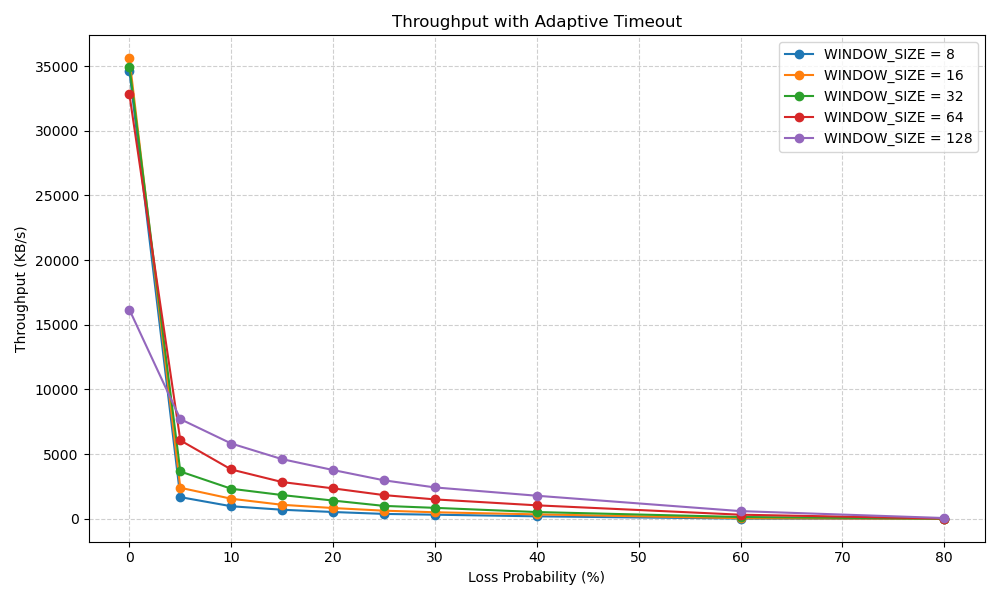
\includegraphics[width=0.65\textwidth]{imgs/04/adaptive-timeout-performance.png}
    \caption{Throughput in funzione della finestra e della probabilità di perdita.}
    \label{fig:throughput_adaptive}
\end{figure}

\subsection{Test Timeout Statico}
Durante l'esecuzione di questo test sono stati utilizzati dei valori della probabilità di perdita nell'intervallo $[0\%, 90\%]$, una dimensione della finestra \lstinlinebg{WINDOW_SIZE} fissa a \lstinlinebg{32} e un timeout statico impostato nel range $[4000 \mu s, 80000 \mu s]$.
Mettendo insieme tutti i risultati ottenuti dai test è stato possibile costruire la seguente tabella:

\begin{table}[htbp]
    \centering
    \renewcommand{\arraystretch}{1.3} % Aumenta spaziatura verticale
    \caption{Throughput in funzione del timeout statico e della probabilità di perdita.}
    \label{tab:throughput_static}
    \begin{tabular}{
        >{\centering\arraybackslash}p{1.2cm}|
        >{\centering\arraybackslash}p{1.5cm}|
        >{\centering\arraybackslash}p{1.6cm}|
        >{\centering\arraybackslash}p{1.6cm}|
        >{\centering\arraybackslash}p{1.6cm}|
        >{\centering\arraybackslash}p{1.6cm}|
        >{\centering\arraybackslash}p{1.6cm}|
        >{\centering\arraybackslash}p{1.6cm}
    }
    \toprule
    \rowcolor{headercolor}
    \multicolumn{2}{c|}{\textbf{Dim. finestra}} & \multicolumn{6}{c}{\textbf{Timeout Statico (in $\boldsymbol{\mu}$s)}} \\
    \rowcolor{headercolor}
    \multicolumn{2}{c|}{\textbf{pari a \textbf{32}}} & \textbf{4000} & \textbf{8000} & \textbf{16000} & \textbf{32000} & \textbf{64000} & \textbf{80000} \\
    \midrule
    
    \multirow{11}{*}{\rotatebox[origin=c]{90}{\textbf{Probabilità di Perdita}}} & 
    \cellcolor{rowcolor1}\textbf{0\%} & 
    \cellcolor{rowcolor1}39653.63 & 
    \cellcolor{rowcolor1}32443.26 & 
    \cellcolor{rowcolor1}28928.45 & 
    \cellcolor{rowcolor1}34412.50 & 
    \cellcolor{rowcolor1}42966.73 & 
    \cellcolor{rowcolor1}36106.52 \\
    
    & \cellcolor{rowcolor2}\textbf{5\%} & 
    \cellcolor{rowcolor2}4727.65 & 
    \cellcolor{rowcolor2}3576.49 & 
    \cellcolor{rowcolor2}2490.50 & 
    \cellcolor{rowcolor2}1277.62 & 
    \cellcolor{rowcolor2}835.57 & 
    \cellcolor{rowcolor2}685.13 \\
    
    & \cellcolor{rowcolor1}\textbf{10\%} & 
    \cellcolor{rowcolor1}3500.83 & 
    \cellcolor{rowcolor1}2502.25 & 
    \cellcolor{rowcolor1}1768.88 & 
    \cellcolor{rowcolor1}909.38 & 
    \cellcolor{rowcolor1}525.79 & 
    \cellcolor{rowcolor1}425.64 \\
    
    & \cellcolor{rowcolor2}\textbf{15\%} & 
    \cellcolor{rowcolor2}2714.11 & 
    \cellcolor{rowcolor2}1914.10 & 
    \cellcolor{rowcolor2}1191.13 & 
    \cellcolor{rowcolor2}655.45 & 
    \cellcolor{rowcolor2}348.69 & 
    \cellcolor{rowcolor2}283.20 \\
    
    & \cellcolor{rowcolor1}\textbf{20\%} & 
    \cellcolor{rowcolor1}2206.86 & 
    \cellcolor{rowcolor1}1512.28 & 
    \cellcolor{rowcolor1}892.03 & 
    \cellcolor{rowcolor1}585.37 & 
    \cellcolor{rowcolor1}267.25 & 
    \cellcolor{rowcolor1}254.48 \\
    
    & \cellcolor{rowcolor2}\textbf{25\%} & 
    \cellcolor{rowcolor2}1694.11 & 
    \cellcolor{rowcolor2}1068.69 & 
    \cellcolor{rowcolor2}690.16 & 
    \cellcolor{rowcolor2}382.73 & 
    \cellcolor{rowcolor2}218.91 & 
    \cellcolor{rowcolor2}164.52 \\
    
    & \cellcolor{rowcolor1}\textbf{30\%} & 
    \cellcolor{rowcolor1}1304.02 & 
    \cellcolor{rowcolor1}926.47 & 
    \cellcolor{rowcolor1}562.95 & 
    \cellcolor{rowcolor1}309.86 & 
    \cellcolor{rowcolor1}170.61 & 
    \cellcolor{rowcolor1}132.60 \\
    
    & \cellcolor{rowcolor2}\textbf{40\%} & 
    \cellcolor{rowcolor2}830.81 & 
    \cellcolor{rowcolor2}578.49 & 
    \cellcolor{rowcolor2}355.41 & 
    \cellcolor{rowcolor2}204.92 & 
    \cellcolor{rowcolor2}108.62 & 
    \cellcolor{rowcolor2}88.31 \\
    
    & \cellcolor{rowcolor1}\textbf{60\%} & 
    \cellcolor{rowcolor1}324.29 & 
    \cellcolor{rowcolor1}221.31 & 
    \cellcolor{rowcolor1}133.52 & 
    \cellcolor{rowcolor1}75.07 & 
    \cellcolor{rowcolor1}39.99 & 
    \cellcolor{rowcolor1}32.43 \\
    
    & \cellcolor{rowcolor2}\textbf{80\%} & 
    \cellcolor{rowcolor2}75.57 & 
    \cellcolor{rowcolor2}50.82 & 
    \cellcolor{rowcolor2}30.73 & 
    \cellcolor{rowcolor2}17.16 & 
    \cellcolor{rowcolor2}9.09 & 
    \cellcolor{rowcolor2}7.36 \\
    
    & \cellcolor{rowcolor1}\textbf{90\%} & 
    \cellcolor{rowcolor1}18.94 & 
    \cellcolor{rowcolor1}12.70 & 
    \cellcolor{rowcolor1}7.62 & 
    \cellcolor{rowcolor1}4.25 & 
    \cellcolor{rowcolor1}2.25 & 
    \cellcolor{rowcolor1}1.35 \\
    \bottomrule
    \multicolumn{8}{r}{Valori espressi in kB/s} \\
    \end{tabular}
\end{table}

Successivamente, grazie ad uno script automatizzato in Python, è stato possibile costruire il grafico mostrato in Fig. \ref{fig:throughput_static}.

\begin{figure}[htbp]
    \centering
    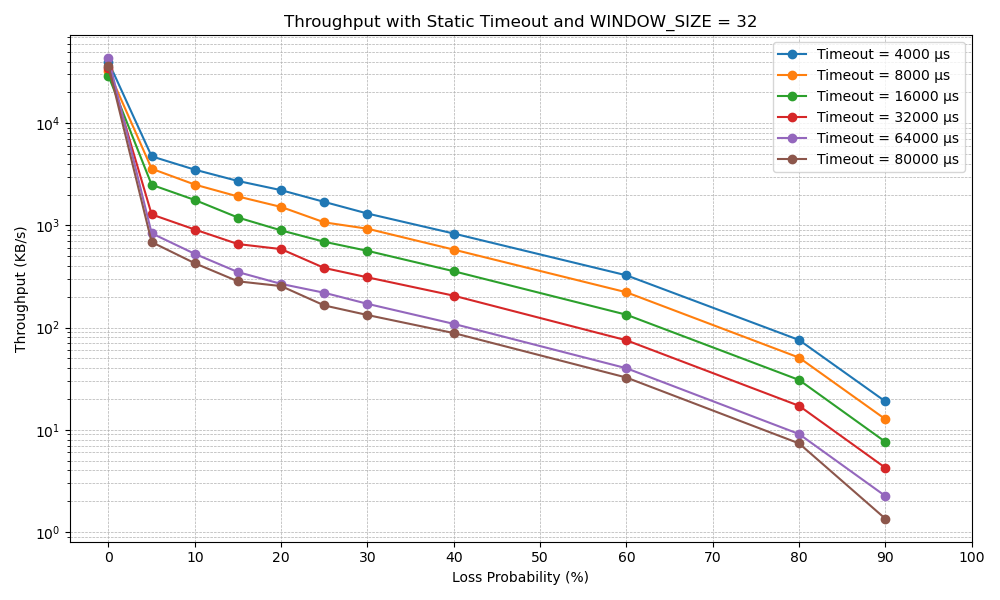
\includegraphics[width=0.65\textwidth]{imgs/04/static-timeout-performance.png}
    \caption{Throughput in funzione del timeout statico e della probabilità di perdita.}
    \label{fig:throughput_static}
\end{figure}

\subsection{Test Timeout Statico \emoji{vs-button} Timeout Adattivo}
Durante l'esecuzione di questo test sono stati riutilizzati i precedenti valori calcolati per il timeout statico e il timeout adattivo e sono stati messi a confronto.
Inoltre è stata aggiunta una colonna relativa alla comulazione di errore per quanto riguarda il timeout adattivo.
Mettendo insieme tutti i risultati ottenuti dai test è stato possibile costruire la seguente tabella:

\begin{table}[htbp]
    \centering
    \renewcommand{\arraystretch}{1.3} % Aumenta spaziatura verticale
    \caption{Confronto throughput fra timeout statico e timeout adattivo.}
    \label{tab:throughput_comparison}
    \begin{tabular}{
        >{\centering\arraybackslash}p{1cm}|
        >{\centering\arraybackslash}p{1.7cm}|
        >{\centering\arraybackslash}p{2.7cm}|
        >{\centering\arraybackslash}p{2cm}|
        >{\centering\arraybackslash}p{1.8cm}|
        >{\centering\arraybackslash}p{1.8cm}|
        >{\centering\arraybackslash}p{1.8cm}
    }
    \toprule
    \rowcolor{headercolor}
    \multicolumn{2}{c|}{\textbf{Dim. finestra}} & 
    \textbf{Cumulazione} & 
    \textbf{Timeout} & 
    \multicolumn{3}{c}{\textbf{Timeout Statici (in $\boldsymbol{\mu}$s)}} \\
    \rowcolor{headercolor}
    \multicolumn{2}{c|}{\textbf{pari a 32}} & \textbf{Errori} & \textbf{Adattivo} & 
    \textbf{8000} & 
    \textbf{32000} & 
    \textbf{80000} \\
    \midrule
    
    \multirow{10}{*}{\rotatebox[origin=c]{90}{\textbf{Probabilità di Perdita}}} &
    \cellcolor{rowcolor1}\textbf{0\%} &
    \cellcolor{rowcolor1}0 &
    \cellcolor{rowcolor1}34971.78 &
    \cellcolor{rowcolor1}32443.26 &
    \cellcolor{rowcolor1}34412.50 &
    \cellcolor{rowcolor1}36106.52 \\
    
    & \cellcolor{rowcolor2}\textbf{5\%} &
    \cellcolor{rowcolor2}34 -- 45 &
    \cellcolor{rowcolor2}3653.44 &
    \cellcolor{rowcolor2}3576.49 &
    \cellcolor{rowcolor2}1277.62 &
    \cellcolor{rowcolor2}685.13 \\
    
    & \cellcolor{rowcolor1}\textbf{10\%} &
    \cellcolor{rowcolor1}53 -- 62 &
    \cellcolor{rowcolor1}2318.92 &
    \cellcolor{rowcolor1}2502.25 &
    \cellcolor{rowcolor1}909.38 &
    \cellcolor{rowcolor1}425.64 \\
    
    & \cellcolor{rowcolor2}\textbf{15\%} &
    \cellcolor{rowcolor2}73 -- 88 &
    \cellcolor{rowcolor2}1831.08 &
    \cellcolor{rowcolor2}1914.10 &
    \cellcolor{rowcolor2}655.45 &
    \cellcolor{rowcolor2}283.20 \\
    
    & \cellcolor{rowcolor1}\textbf{20\%} &
    \cellcolor{rowcolor1}89 -- 108 &
    \cellcolor{rowcolor1}1404.64 &
    \cellcolor{rowcolor1}1512.28 &
    \cellcolor{rowcolor1}585.37 &
    \cellcolor{rowcolor1}254.48 \\
    
    & \cellcolor{rowcolor2}\textbf{25\%} &
    \cellcolor{rowcolor2}128 -- 138 &
    \cellcolor{rowcolor2}993.31 &
    \cellcolor{rowcolor2}1068.69 &
    \cellcolor{rowcolor2}382.73 &
    \cellcolor{rowcolor2}164.52 \\
    
    & \cellcolor{rowcolor1}\textbf{30\%} &
    \cellcolor{rowcolor1}164 -- 181 &
    \cellcolor{rowcolor1}842.40 &
    \cellcolor{rowcolor1}926.47 &
    \cellcolor{rowcolor1}309.86 &
    \cellcolor{rowcolor1}132.60 \\
    
    & \cellcolor{rowcolor2}\textbf{40\%} &
    \cellcolor{rowcolor2}257 -- 280 &
    \cellcolor{rowcolor2}518.07 &
    \cellcolor{rowcolor2}578.49 &
    \cellcolor{rowcolor2}204.92 &
    \cellcolor{rowcolor2}88.31 \\
    
    & \cellcolor{rowcolor1}\textbf{60\%} &
    \cellcolor{rowcolor1}693 -- 715 &
    \cellcolor{rowcolor1}135.48 &
    \cellcolor{rowcolor1}221.31 &
    \cellcolor{rowcolor1}75.07 &
    \cellcolor{rowcolor1}32.43 \\
    
    & \cellcolor{rowcolor2}\textbf{80\%} &
    \cellcolor{rowcolor2}2980 -- 3082 &
    \cellcolor{rowcolor2}7.49 &
    \cellcolor{rowcolor2}50.82 &
    \cellcolor{rowcolor2}17.16 &
    \cellcolor{rowcolor2}7.36 \\
    \bottomrule
    \multicolumn{7}{r}{Valori espressi in kB/s} \\
    \end{tabular}
\end{table}

Successivamente, grazie ad uno script automatizzato in Python, è stato possibile costruire il grafico mostrato in Fig. \ref{fig:throughput_adaptive_vs_static}.

\begin{figure}[htbp]
    \centering
    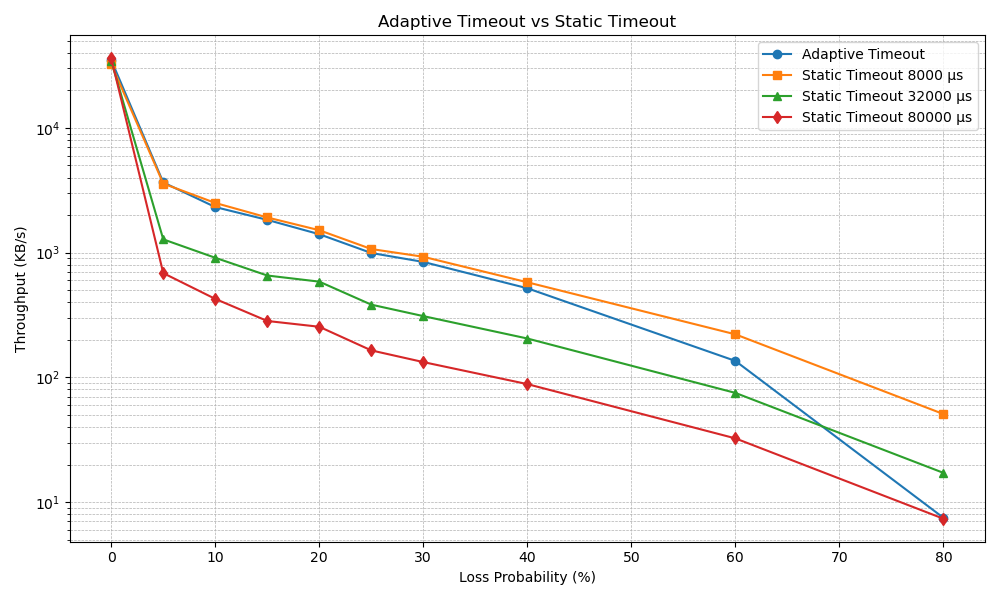
\includegraphics[width=0.65\textwidth]{imgs/04/static-vs-adaptive-timeout-performance.png}
    \caption{Confronto throughput fra timeout statico e timeout adattivo.}
    \label{fig:throughput_adaptive_vs_static}
\end{figure}

\subsection{Test cumulazione degli errori}
Per questo test sono stati utilizzati i valori della comulazione di errore calcolati per il timeout statico e il timeout adattivo e sono stati messi a confronto.
Questi errori vengono memorizzati tramite la variabile \lstinlinebg{max_errors} che tiene traccia del numero massimo di errori consecutivi che si possono verificare durante il trasferimento di un file.
Mettendo insieme tutti i risultati ottenuti dai test è stato possibile costruire la seguente tabella:

\begin{table}[htbp]
    \centering
    \renewcommand{\arraystretch}{1.3} % Aumenta spaziatura verticale
    \caption{Comulazione degli errori in funzione della probabilità di perdita.}
    \label{tab:throughput_error}
    \begin{tabular}{
        >{\centering\arraybackslash}p{1cm}|
        >{\centering\arraybackslash}p{1.75cm}|
        >{\centering\arraybackslash}p{1.75cm}|
        >{\centering\arraybackslash}p{1.75cm}|
        >{\centering\arraybackslash}p{1.75cm}|
        >{\centering\arraybackslash}p{1.75cm}|
        >{\centering\arraybackslash}p{1.75cm}
    }
    \toprule
    \rowcolor{headercolor}
    \multicolumn{2}{c|}{\textbf{Comulazione}} & \multicolumn{5}{c}{\textbf{Dimensione della Finestra}} \\
    \rowcolor{headercolor}
    \multicolumn{2}{c|}{\textbf{Errori}} & \textbf{8} & \textbf{16} & \textbf{32} & \textbf{64} & \textbf{128} \\
    \midrule
    
    \multirow{10}{*}{\rotatebox[origin=c]{90}{\textbf{Probabilità di Perdita}}} & 
    \cellcolor{rowcolor1}\textbf{0\%} & 
    \cellcolor{rowcolor1}0 & 
    \cellcolor{rowcolor1}0 & 
    \cellcolor{rowcolor1}0 & 
    \cellcolor{rowcolor1}0 & 
    \cellcolor{rowcolor1}6 \\
    
    & \cellcolor{rowcolor2}\textbf{5\%} & 
    \cellcolor{rowcolor2}85 -- 99 & 
    \cellcolor{rowcolor2}56 -- 67 & 
    \cellcolor{rowcolor2}34 -- 35 & 
    \cellcolor{rowcolor2}24 -- 30 & 
    \cellcolor{rowcolor2}13 -- 20 \\
    
    & \cellcolor{rowcolor1}\textbf{10\%} & 
    \cellcolor{rowcolor1}127 -- 155 & 
    \cellcolor{rowcolor1}86 -- 92 & 
    \cellcolor{rowcolor1}53 -- 62 & 
    \cellcolor{rowcolor1}32 -- 42 & 
    \cellcolor{rowcolor1}23 -- 25 \\
    
    & \cellcolor{rowcolor2}\textbf{15\%} & 
    \cellcolor{rowcolor2}184 -- 209 & 
    \cellcolor{rowcolor2}122 -- 153 & 
    \cellcolor{rowcolor2}73 -- 88 & 
    \cellcolor{rowcolor2}43 -- 51 & 
    \cellcolor{rowcolor2}26 --30 \\
    
    & \cellcolor{rowcolor1}\textbf{20\%} & 
    \cellcolor{rowcolor1}240 -- 279 & 
    \cellcolor{rowcolor1}169 -- 189 & 
    \cellcolor{rowcolor1}89 -- 108 & 
    \cellcolor{rowcolor1}62 -- 69 & 
    \cellcolor{rowcolor1}32 -- 39 \\
    
    & \cellcolor{rowcolor2}\textbf{25\%} & 
    \cellcolor{rowcolor2}331 -- 348 & 
    \cellcolor{rowcolor2}207 -- 222 & 
    \cellcolor{rowcolor2}128 -- 138 & 
    \cellcolor{rowcolor2}74 -- 82 & 
    \cellcolor{rowcolor2}42 -- 48 \\
    
    & \cellcolor{rowcolor1}\textbf{30\%} & 
    \cellcolor{rowcolor1}444 -- 472 & 
    \cellcolor{rowcolor1}285 -- 297 & 
    \cellcolor{rowcolor1}164 -- 181 & 
    \cellcolor{rowcolor1}98 -- 116 & 
    \cellcolor{rowcolor1}55 -- 61 \\
    
    & \cellcolor{rowcolor2}\textbf{40\%} & 
    \cellcolor{rowcolor2}681 -- 742 & 
    \cellcolor{rowcolor2}453 -- 477 & 
    \cellcolor{rowcolor2}257 -- 280 & 
    \cellcolor{rowcolor2}151 -- 163 & 
    \cellcolor{rowcolor2}87 -- 92 \\
    
    & \cellcolor{rowcolor1}\textbf{60\%} & 
    \cellcolor{rowcolor1}1889 -- 1932 & 
    \cellcolor{rowcolor1}1202 -- 1230 & 
    \cellcolor{rowcolor1}693 -- 715 & 
    \cellcolor{rowcolor1}374 -- 421 & 
    \cellcolor{rowcolor1}140 -- 218 \\
    
    & \cellcolor{rowcolor2}\textbf{80\%} & 
    \cellcolor{rowcolor2}7963 -- 8548 & 
    \cellcolor{rowcolor2}5028 -- 5507 & 
    \cellcolor{rowcolor2}2980 -- 3082 & 
    \cellcolor{rowcolor2}1682 -- 1844 & 
    \cellcolor{rowcolor2}899 -- 1150 \\
    \bottomrule
    \end{tabular}
\end{table}

Successivamente, grazie ad uno script automatizzato in Python, è stato possibile costruire i grafici mostrati in Fig. \ref{fig:throughput_error_static} e Fig. \ref{fig:throughput_error_adaptive}, dove per la comulazione degli errori nel caso del timeout adattivo è stata considerata la colonna della Tabella \ref{tab:throughput_comparison}.

\begin{figure}[htbp]
    \centering
    \begin{minipage}{0.49\textwidth}
        \centering
        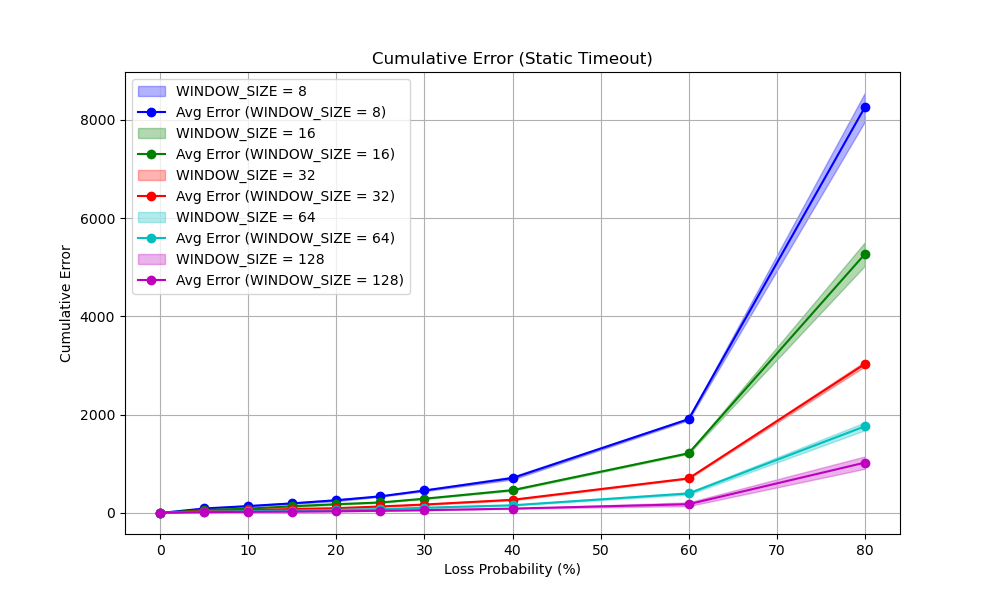
\includegraphics[width=\textwidth]{imgs/04/static-cumulative-error.png}
        \caption{Comulazione degli errori per il timeout statico.}
        \label{fig:throughput_error_static}
    \end{minipage}
    \hfill
    \begin{minipage}{0.49\textwidth}
        \centering
        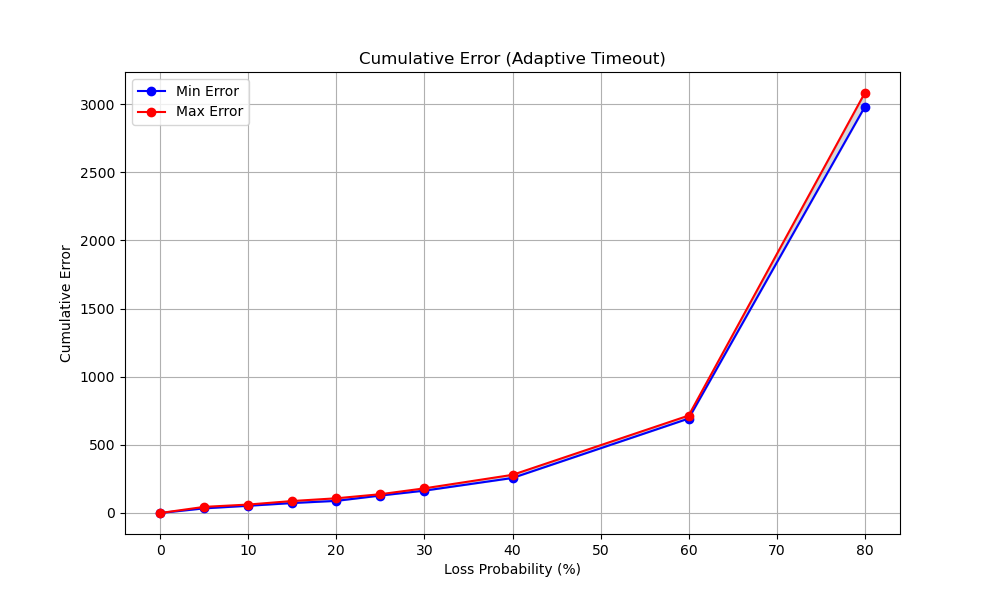
\includegraphics[width=\textwidth]{imgs/04/adaptive-cumulative-error.png}
        \caption{Comulazione degli errori per il timeout adattivo.}
        \label{fig:throughput_error_adaptive}
    \end{minipage}
\end{figure}

\section{Test per l'integrità dei file trasferiti \emoji{snake}}
Infine è stato svolto un test per verificare l'integrità dei file trasferiti.
Per fare ciò è stato creato uno script in Python (presente nella directory \lstinlinebg{tests/}) che confronta il file originale e quello trasferito, verificando che siano identici.
Prima di tutto, il programma calcola l'hash dei file utilizzando un algoritmo di hashing sicuro, come SHA-256, che permette di rilevare rapidamente eventuali differenze nel contenuto.
L'hash viene calcolato leggendo il file a blocchi per ottimizzare l'efficienza anche con file di grandi dimensioni.
Se gli hash di due file sono identici, il programma esegue un ulteriore confronto byte per byte per essere completamente sicuro che i file siano uguali.
Il funzionamento si estende a due directory specificate dall'utente, denominate di default con \lstinlinebg{client-files/} e \lstinlinebg{server-files/}.
Il programma analizza il contenuto di entrambe le directory, confrontando i file con lo stesso nome.
Se due file hanno lo stesso nome ma contenuti differenti, il programma segnala la differenza, evidenziandola in rosso nel terminale.
Se, invece, i file sono uguali, viene indicato un messaggio in verde, confermando che i file sono identici.
Inoltre, il programma elenca anche i file che sono presenti solo in una delle due directory, fornendo un riepilogo completo delle differenze.

\subsection{Esempio di funzionamento}
Per esemplificare il funzionamento dello script, può essere usato il file di testo \lstinlinebg{GuidaC.txt}.
Immaginando che questo file sia stato inviato dal cliente al server (o viceversa).
Per eseguire lo script è sufficiente accedere alla root directory del progetto (ovvero \lstinlinebg{spqr/}) e lanciare il seguente comando:

\begin{lstlisting}[numbers=none]
python tests/integrity-consistency.py
\end{lstlisting}

Un esempio di output dello script è il seguente:

\begin{lstlisting}[numbers=none]
The files "GuidaC.txt" inside "./client-files/" and "./server-files/" are the same.
\end{lstlisting}
